\documentclass[a4paper,12pt]{article}

\usepackage{TPUstyle}

\graphicspath{ {../images/wheel_dynamics} }

\begin{document}

\begin{lemma}
    Описание кинематики колеса.

    Исходные величины (рисунок \ref{fig:lemma1}, направление стрелок показывают положительное направление): \\
    \(\alpha_i\) -- угол между осью \(OX\) и \(OK_i\), характеризует угол положения колеса относительно центра робота; \\
    \(\beta_i\) -- угол поворота колеса в пространстве, угол между \(OX\) и \(M_i\); \\
    \(\sigma_i\) -- угол между \(F_i\) (\(w_i\)) колеса и \(M_i\).

    \begin{figure}[H]
        \centering
        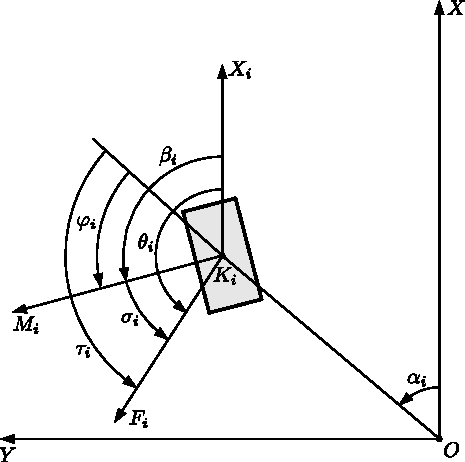
\includegraphics[width=0.6\textwidth]{lemma1.pdf}
        \caption{Определение углов}
        \label{fig:lemma1}
    \end{figure}

    Определить:
    \begin{itemize}
        \item угол \(\phi_i\) между \(OK_i\) и \(M_i\);
        \item угол \(\theta_i\) между \(OX_i\) и \(F_i\).
    \end{itemize}

    \[
        \phi_i = \beta_i - \alpha_i
    ,\]
    \[
        \theta_i = \beta_i + \sigma_i    
    .\] 
\end{lemma}

\begin{lemma}
    Определение сил и моментов, действующих от колеса.

    Дано:
    \begin{enumerate}
        \item \(F_i\) -- сила, создаваемая колесом;
        \item углы \(\alpha_i, \beta_i, \sigma_i\);
        \item \(b_i\) -- расстояние между \(O\) и \(K_i\).
    \end{enumerate}

    \begin{figure}[H]
        \centering
        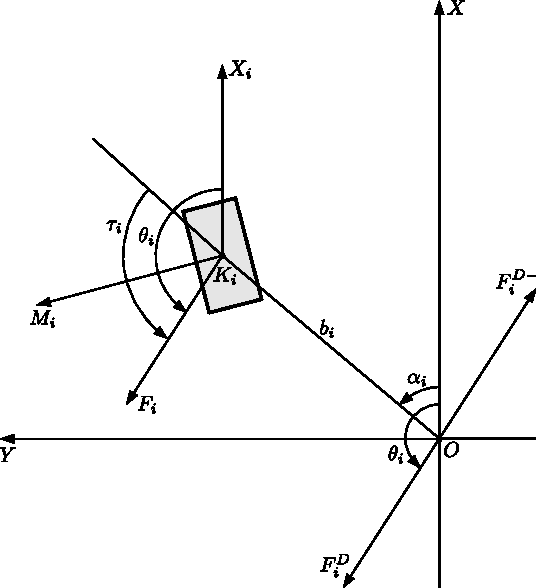
\includegraphics[width=0.6\textwidth]{lemma2.pdf}
        \caption{Определение углов}
        \label{fig:lemma2}
    \end{figure}

    Проекции \(F_i^D\)
    \[
        F_{i x}^D = F_i^D \cos \theta_i = F_i^D \cos\left( \beta_i + \sigma_i \right)
    ,\]
    \[
        F_{i y}^D = F_i^D \sin \theta_i = F_i^D \sin\left( \beta_i + \sigma_i \right)
    .\]

    Момент вращения
    \[
        M_\text{вр} = F_i b_i \sin \tau_i = F_i b_i \sin\left( \sigma_i + \phi_i \right) = F_i b_i \sin\left( \sigma_i + \beta_i - \alpha_i \right) 
    .\]
\end{lemma}

\end{document}